\documentclass[12pt,letterpaper]{article}
\usepackage[utf8]{inputenc}
\usepackage[spanish]{babel}
\usepackage{graphicx}
\usepackage[left=2cm,right=2cm,top=2cm,bottom=2cm]{geometry}
\usepackage{graphicx} % figuras
% \usepackage{subfigure} % subfiguras
\usepackage{float} % para usar [H]
\usepackage{amsmath}
%\usepackage{txfonts}
\usepackage{stackrel} 
\usepackage{multirow}
\usepackage{enumerate} % enumerados
\renewcommand{\labelitemi}{$-$}
\renewcommand{\labelitemii}{$\cdot$}
% \author{}
% \title{Caratula}
\begin{document}

% Fancy Header and Footer
% \usepackage{fancyhdr}
% \pagestyle{fancy}
% \cfoot{}
% \rfoot{\thepage}
%

% \usepackage[hidelinks]{hyperref} % CREA HYPERVINCULOS EN INDICE

% \author{}
\title{Caratula}

\begin{titlepage}
\begin{center}
\large{UNIVERSIDAD PRIVADA DE TACNA}\\
\vspace*{-0.025in}
\begin{figure}[htb]
\begin{center}

\includegraphics[width=7cm]{./images/logo}
\end{center}
\end{figure}
\vspace*{0.15in}
INGENIERIA DE SISTEMAS  \\

\vspace*{0.3in}
\begin{large}
\textbf{TITULO:} \\
\end{large}

\vspace*{0.1in}
\begin{Large}
\textbf{ Modelando Datos en Power BI} \\

\end{Large}

\vspace*{0.3in}
\begin{Large}
\textbf{CURSO:} \\
\end{Large}

\vspace*{0.1in}
\begin{large}
INTELIGENCIA DE NEGOCIOS\\
\end{large}

\vspace*{0.3in}
\begin{Large}
\textbf{DOCENTE:} \\
\end{Large}

\vspace*{0.1in}
\begin{large}
 Ing. Patrick Jose Cuadros Quiroga\\
\end{large}

\vspace*{0.4in}
\vspace*{0.1in}
\begin{large}
\textbf{INTEGRANTES:} \\
\begin{flushleft}
Escalante Alanoca Jesus Humberto\hfill	(2015050641)\\

\centering  %CENTRA UN TEXTO
\vspace*{0.9in}
\begin{large}
Tacna\\ 11-09-2019
\end{large}

\end{flushleft}
\end{large}
\end{center}

\end{titlepage}


\tableofcontents % INDICE
\thispagestyle{empty} % INDICE SIN NUMERO
\newpage
\setcounter{page}{1} % REINICIAR CONTADOR DE PAGINAS DESPUES DEL INDICE


\section{ Crear Relaciones}
\subsection{ Relaciones automáticas}

\begin{center}
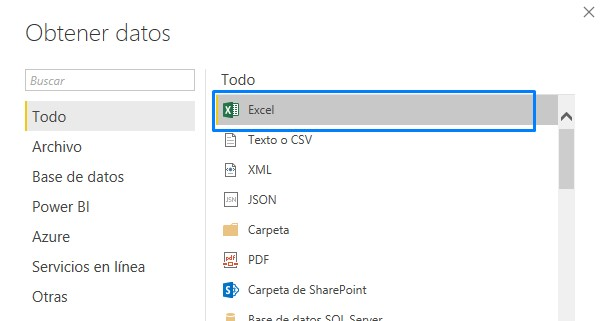
\includegraphics[width=\columnwidth]{images/task1/task1-01}\newline
\end{center}

\begin{center}
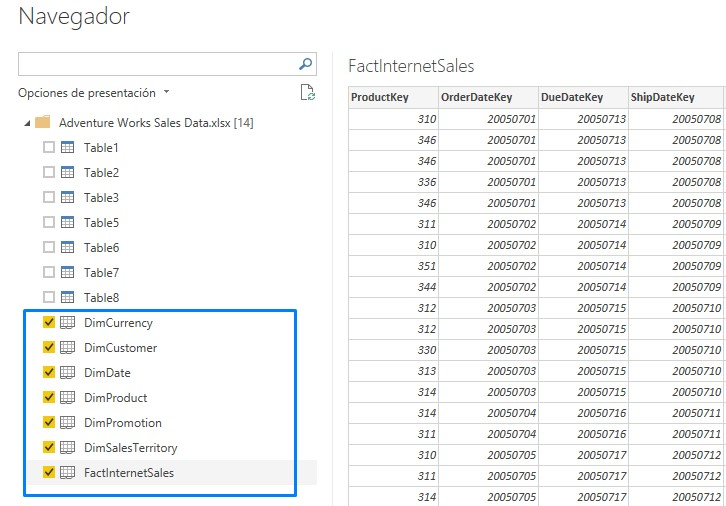
\includegraphics[width=\columnwidth]{images/task1/task1-02}\newline
\end{center}

\begin{center}
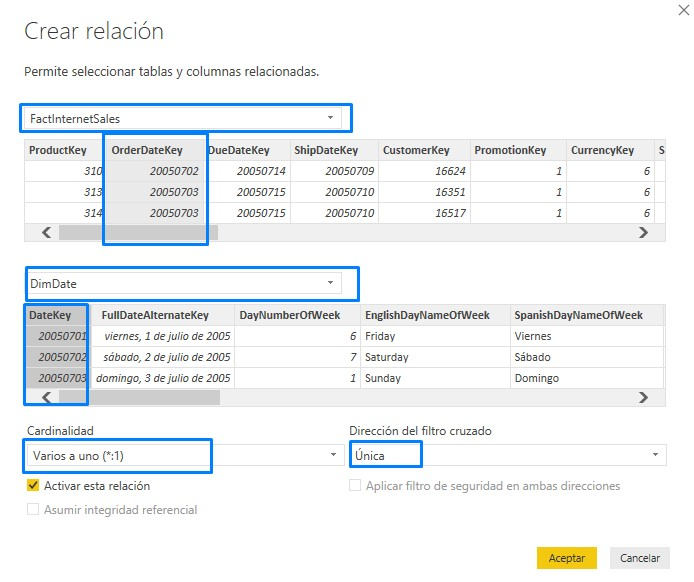
\includegraphics[width=\columnwidth]{images/task1/task1-03}\newline
\end{center}

\begin{center}
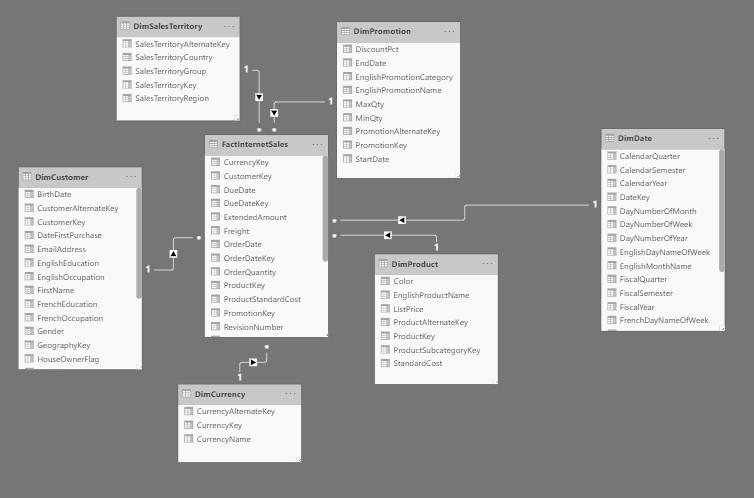
\includegraphics[width=\columnwidth]{images/task1/task1-04}\newline
\end{center}

\subsection{ Relaciones manuales}

\begin{center}
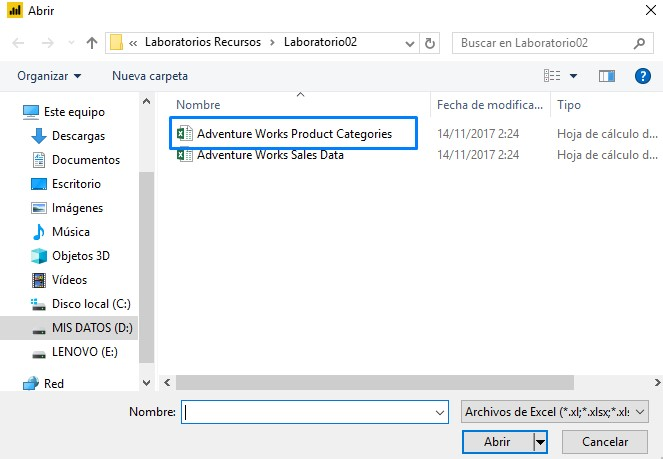
\includegraphics[width=\columnwidth]{images/task2/task2-01}\newline
\end{center}

\begin{center}
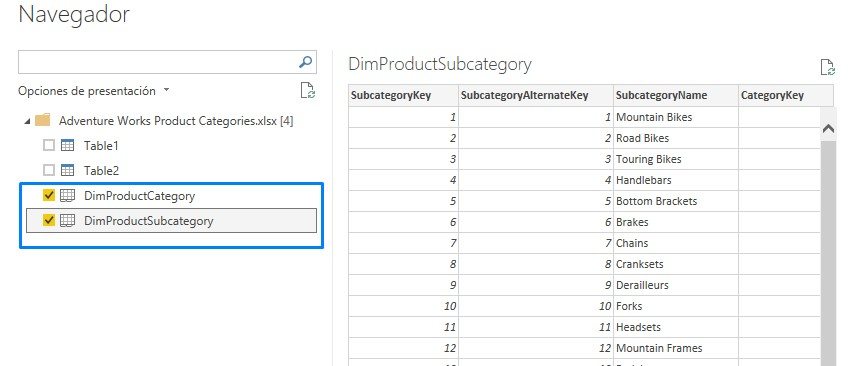
\includegraphics[width=\columnwidth]{images/task2/task2-02}\newline
\end{center}


\begin{center}
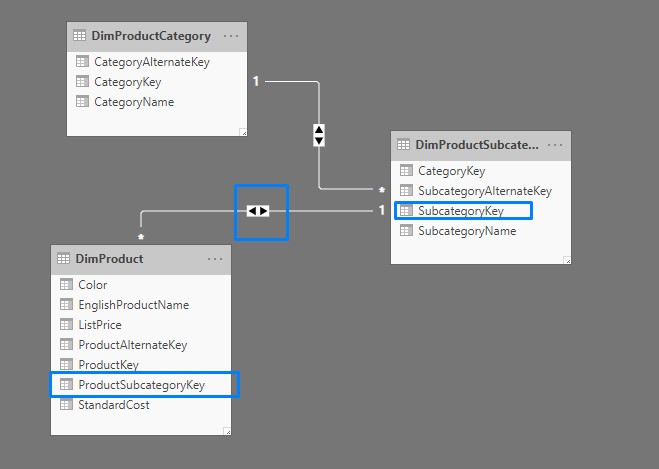
\includegraphics[width=\columnwidth]{images/task2/task2-06}\newline
\end{center}
\section{ Cálculos}
\subsection{ Añadir una columna calculada}


\begin{center}
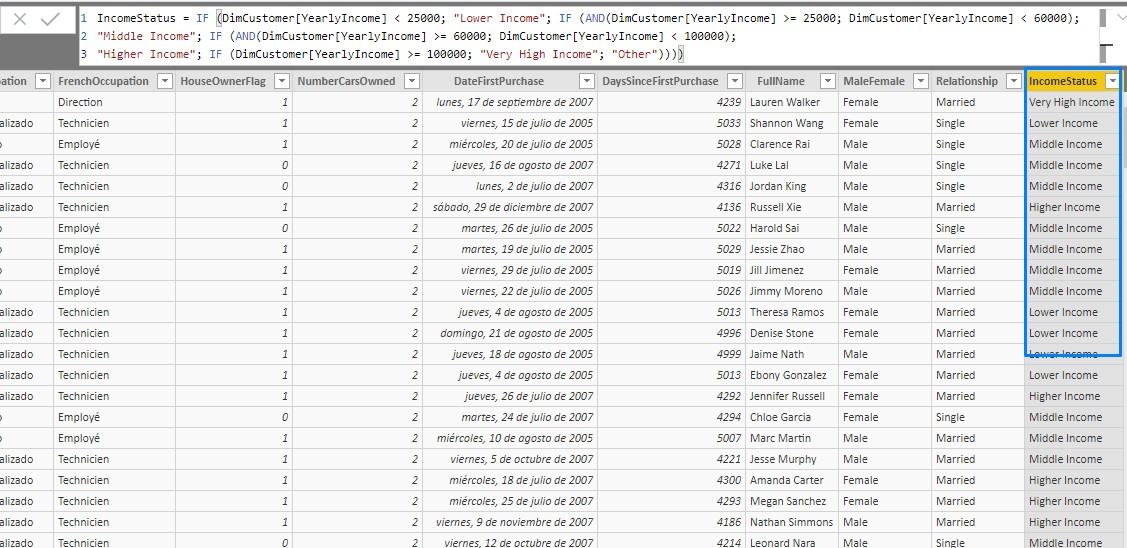
\includegraphics[width=\columnwidth]{images/task3/task3-02}\newline
\end{center}

\begin{center}
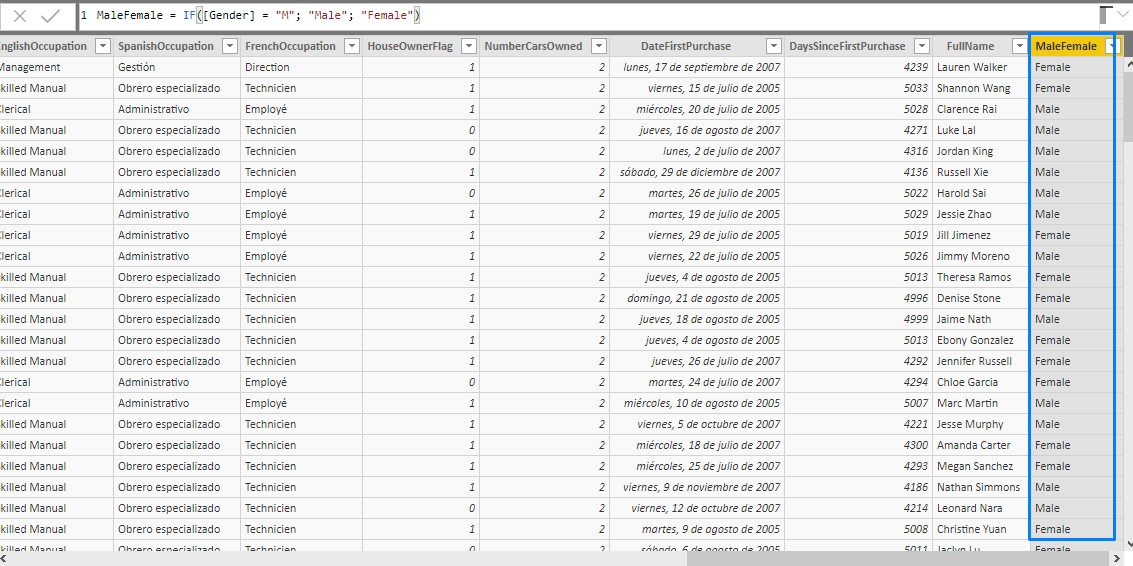
\includegraphics[width=\columnwidth]{images/task3/task3-05}\newline
\end{center}

\begin{center}
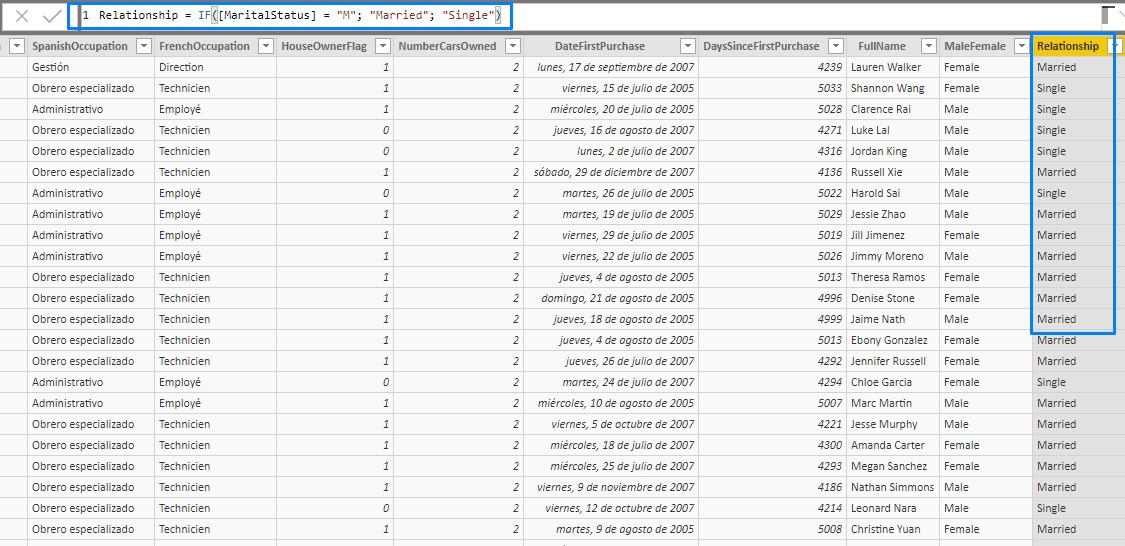
\includegraphics[width=\columnwidth]{images/task3/task3-06}\newline
\end{center}

\begin{center}
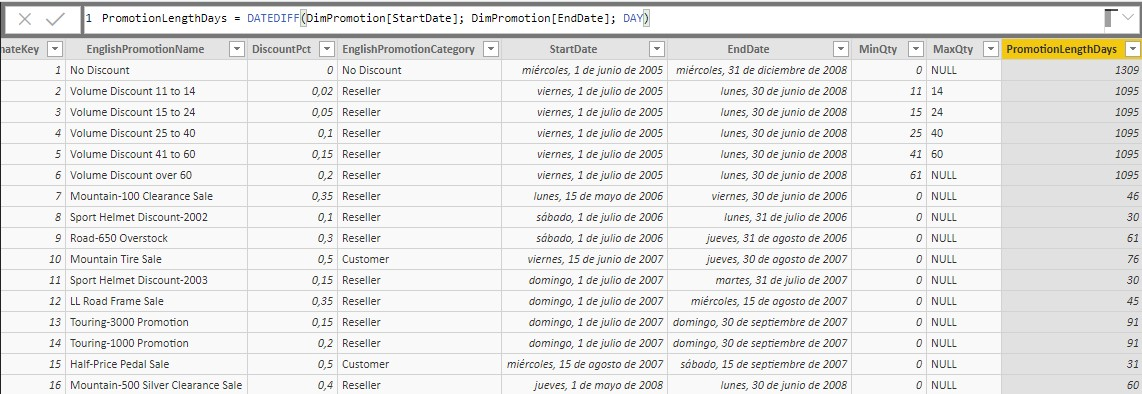
\includegraphics[width=\columnwidth]{images/task3/task3-08}\newline
\end{center}

\end{document}